\paragraph{Задание 1 Вариант 1} \hspace{0pt}

Применить паттерн абстрактная фабрика при построении схемы из простых графических объектов.
Продукты фабрики: прямоугольник, линия, овал, текст.

\begin{figure}[!htb]
    \centering
    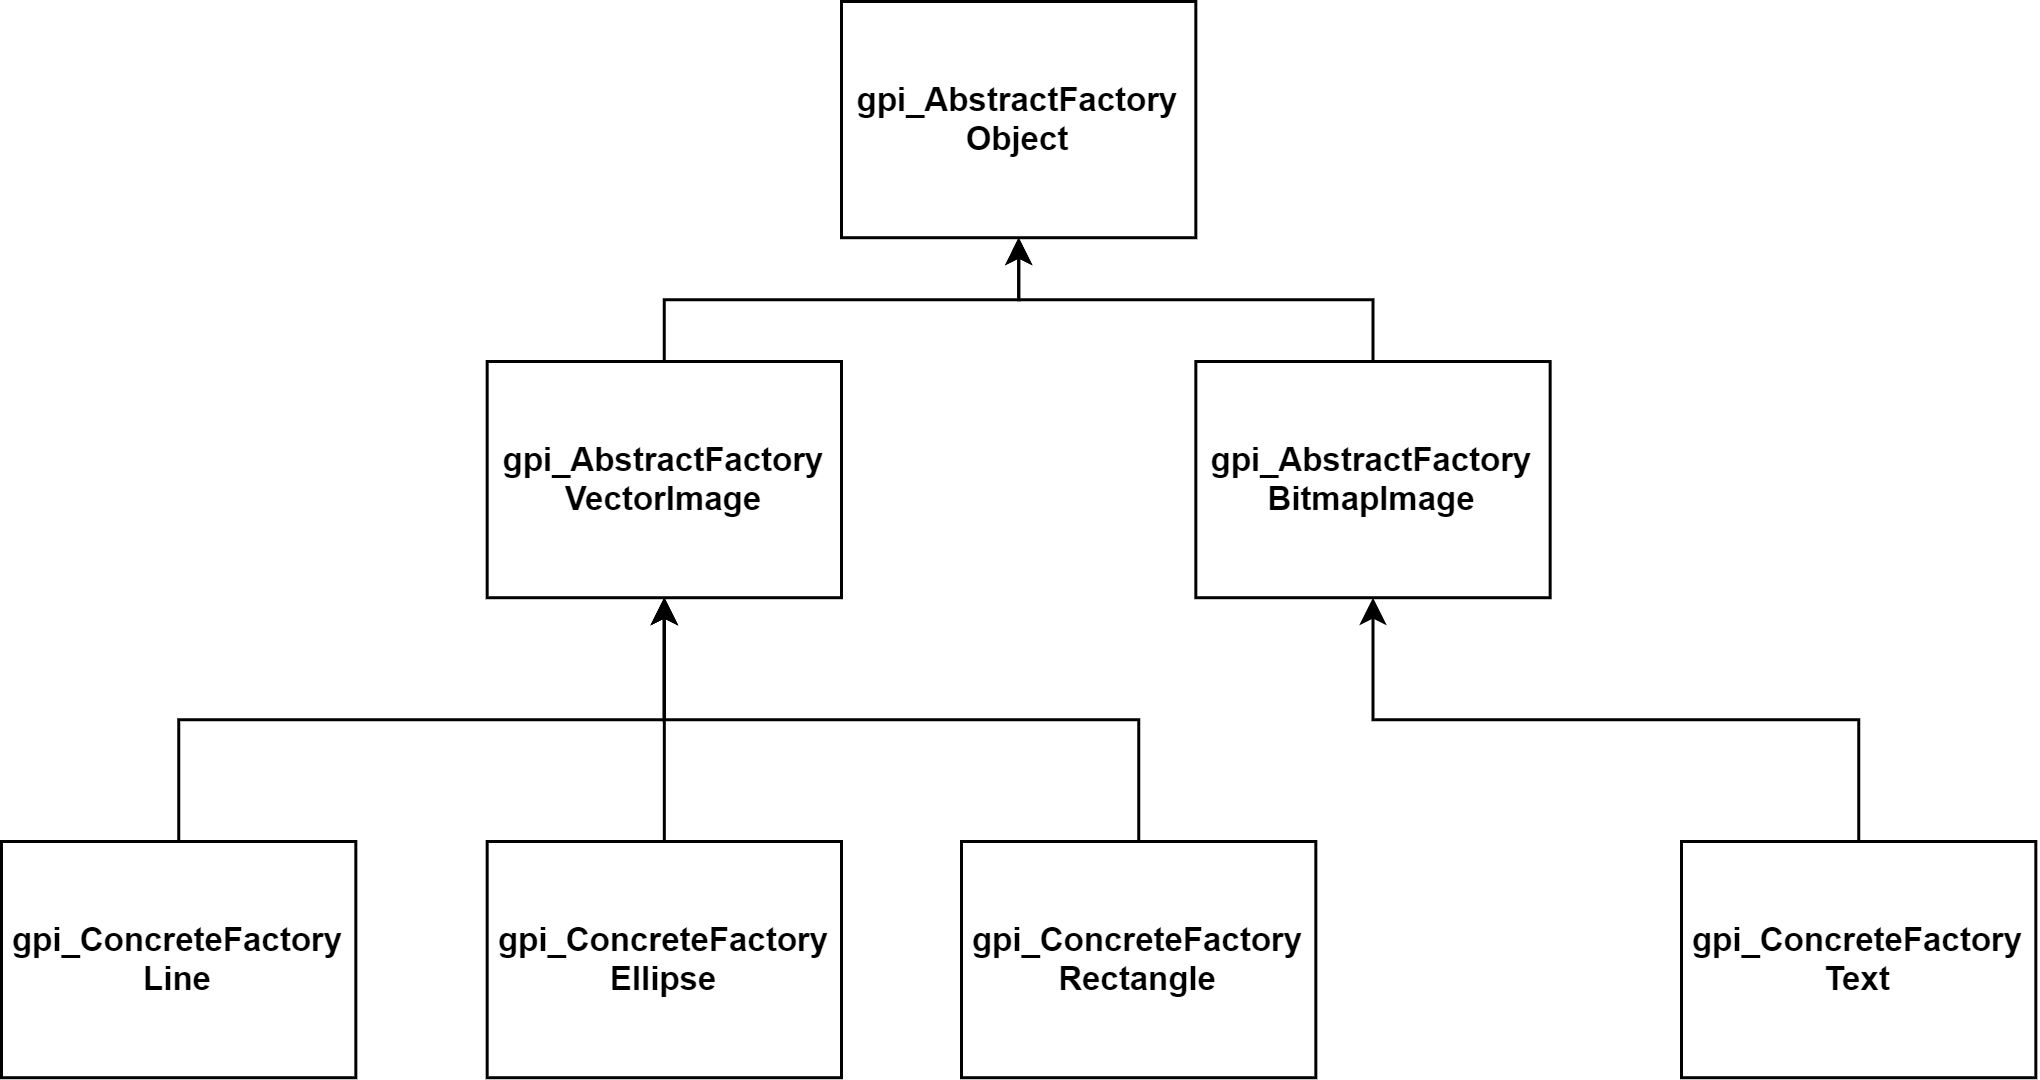
\includegraphics[width=16cm]
        {_assets/gpi_ootpisp5_lab8_task_1_1.png}
    \caption{Диаграмма наследования классов}
\end{figure}

\lstinputlisting[language=csh, name=Program.cs,]
{../gpi_ootpisp5_lab8_task_1_1/gpi_ootpisp5_lab8_task_1_1/Program.cs}

\lstinputlisting[language=csh, name=gpi_AbstractFactoryObject.cs,]
{../gpi_ootpisp5_lab8_task_1_1/gpi_ootpisp5_lab8_task_1_1/gpi_AbstractFactoryObject.cs}

\lstinputlisting[language=csh, name=gpi_AbstractFactoryBitmapImage.cs,]
{../gpi_ootpisp5_lab8_task_1_1/gpi_ootpisp5_lab8_task_1_1/gpi_AbstractFactoryBitmapImage.cs}

\lstinputlisting[language=csh, name=gpi_AbstractFactoryVectorImage.cs,]
{../gpi_ootpisp5_lab8_task_1_1/gpi_ootpisp5_lab8_task_1_1/gpi_AbstractFactoryVectorImage.cs}

\lstinputlisting[language=csh, name=gpi_ConcreteFactoryText.cs,]
{../gpi_ootpisp5_lab8_task_1_1/gpi_ootpisp5_lab8_task_1_1/gpi_ConcreteFactoryText.cs}

\lstinputlisting[language=csh, name=gpi_ConcreteFactoryLine.cs,]
{../gpi_ootpisp5_lab8_task_1_1/gpi_ootpisp5_lab8_task_1_1/gpi_ConcreteFactoryLine.cs}

\lstinputlisting[language=csh, name=gpi_ConcreteFactoryRectangle.cs,]
{../gpi_ootpisp5_lab8_task_1_1/gpi_ootpisp5_lab8_task_1_1/gpi_ConcreteFactoryRectangle.cs}

\lstinputlisting[language=csh, name=gpi_ConcreteFactoryEllipse.cs,]
{../gpi_ootpisp5_lab8_task_1_1/gpi_ootpisp5_lab8_task_1_1/gpi_ConcreteFactoryEllipse.cs}

\lstinputlisting[name=Console out,]
{_assets/gpi_ootpisp5_lab8_task_1_1.exe.txt}
